\chapter{经验研究}



为了了解已有漏洞数据库中开源软件漏洞补丁的质量和特征,本文开展了一项针对当前\tocheck{高质量}漏洞数据库的经验研究。本章节将介绍经验研究的设计、\tocheck{数据收集与解析}以及经验研究的结果分析。


\section{研究设计}
\subsection{研究问题}
\begin{itemize}[leftmargin=*]
    \item \textbf{RQ1 覆盖率分析:}漏洞库中,漏洞补丁信息的覆盖度如何?即:有多少漏洞包含补丁信息?(Sec. \ref{sec:coverage})
    \item \textbf{RQ2 一致性分析:}不用漏洞库间,漏洞补丁信息的一直性如何?即:有多少漏洞在漏洞数据库中具有相同的补丁?(Sec. \ref{sec:consistency})
    \item \textbf{RQ3 补丁类型分析:}漏洞补丁的类型有哪些? (Sec. \ref{sec:type})
    \item \textbf{RQ4 补丁映射分析:}漏洞与其补丁在数量上的映射关系是怎样的? (Sec. \ref{sec:cardinality})
    \item \textbf{RQ5 补丁准确性分析:}漏洞库中,漏洞的补丁信息准确度如何? (Sec. \ref{sec:accuracy})
\end{itemize}
    
其中,RQ1可用来衡量不同漏洞数据库中开源软件漏洞的补丁缺失程度,RQ2用来量化不同漏洞数据库中漏洞补丁的不一致程度,RQ3和RQ4用来统计常见的补丁类型以及开源漏洞及其补丁之间的映射关系,RQ5用以评估不同漏洞数据库中漏洞补丁信息的准确性。总的来说,RQ1、RQ2和RQ5的结果旨在从不同的角度评估补丁质量,并挖掘出对自动化补丁\tocheck{识别}方法的需求;RQ3和RQ4旨在从不同角度捕捉开源软件漏洞补丁的特征,并为自动化补丁\tocheck{识别}方法的设计提供\tocheck{启发}。

\subsection{评估标准【todo】}
precision、recall。。。

\section{数据准备}\label{sec:preparation}
\subsection{漏洞数据库选择}
本文前期调研了来自安全社区、工业界和学术界的漏洞数据库。在该章节的经验研究中,本文首先排除了来自安全社区的数据库(例如,CVE和NVD)。因为它们没有结构化的补丁信息,而补丁信息多是隐藏在参考链接中;此外,CVE和NVD数据库不仅仅包含开源软件漏洞,还包括闭源软件、系统及硬件相关的漏洞。
本文还排除了来自学术界的数据集\cite{ponta2019manually,fan2020ac,jimenez2018enabling,gkortzis2018vulinoss,namrud2019androvul,li2017large,liu2020large,antal2020exploring},这是因为这些数据集中的漏洞通常限定于特定程序语言(例如:Python、Java)而非面向所有开源软件,此外,由于长期缺乏维护,这些漏洞数据集缺失较新的漏洞数据。


本文关注到BlackDuck\cite{blackduck}、WhiteSource\cite{whitesource}、Veracode\cite{veracode}和Snyk\cite{snyk}四家公司提供软件成分分析(Software Composition Analysis)服务,该服务识别当前软件系统中使用的开源成本(即:第三方库),并报告开源成分相关的漏洞。因此,这四家公司需要构建尽可能完整且包含详细漏洞信息的漏洞库作为基础,本文便首先将这四家公司的漏洞数据库作为研究对象。进一步调研发现,某些公司并未公开漏洞数据库,或是公开的信息中不包含漏洞的补丁信息。最终,本文选定Veracode和Snyk的漏洞数据库作为研究对象,下文中简称为:$DB_A$和$DB_B$。


\begin{itemize}[leftmargin=*]
\item\textbf{Black Duck:}该公司的安全公告中共包含157,000多个漏洞,涵盖90多种编程语言。其中,数千个漏洞尚未被NVD收录。这些漏洞信息有特定的专家团队进行维护,以确保漏洞数据的完整性和准确性。然而,157,000多个漏洞中开源漏洞的具体数量并未公开,且具体的漏洞信息也并未公开。
\item\textbf{Sonatype:} 该公司声称:\textit{"OSS Index is a free catalogue of open source components and scanning tools to help developers identify vulnerabilities, understand risk, and keep their software safe."} Sonatype的OSS索引支持20多个生态系统(即:Maven、npm、Go、PyPI等)。该公司的漏洞公告包含:漏洞描述、受漏洞影响的组件和版本、CVSS向量和参考链接等信息\footnote{https://ossindex.sonatype.org}。
\item\textbf{WhiteSource:}该公司从NVD及其他安全公告平台和问题追踪系统(issue tracking system)中收集的漏洞超过175,000个,涵盖200多种编程语言。
\item\textbf{Veracode:}该公司的漏洞数据库涵盖10多种编程语言相关的18,000多个漏洞\tocheck{链接},公开的漏洞信息包括:受漏洞影响的组件和版本范围、库修复说明、参考资料等。
\item\textbf{Snyk:}该公司的漏洞数据库\footnote{https://snyk.io/product/vulnerability-database/}是由经验丰富的安全研究团队持续维护,通过关注安全公告、Jira issue报告,Github commits等方式自动识别安全漏洞相关的报告。该公司的数据库涵盖超过10个编程语言生态系统,如:Maven、npm、Go、Composer等。该数据库提供漏洞的详细信息,包括:受漏洞影响的组件、版本范围、修复方法、参考链接等\footnote{https://snyk.io/vuln}。
% \item \textbf{Gitlab Security} GitLab 咨询数据库是 Gitlab 依赖扫描器\footnote{https://docs.gitlab.com/ee/user/application\_security/dependency\_scanning/index.html} 的基础。目前涵盖了 6000 多个 CVE 条目和 8 个生态系统(即 Nuget、Conan、Maven 等)。提供了详细信息,例如描述、受影响的组件和版本、解决方案和参考。
\end{itemize}



\subsection{广度数据集构建}
为了量化分析漏洞数据库中补丁的缺失程度以及不同数据库间补丁的不一致性(即:RQ1和RQ2),本文从$DB_A$和$DB_B$中获取了所有开源软件漏洞,构建了一个开源软件漏洞的广度数据集。截至2020年4月7日,分别从$DB_A$和$DB_B$中获取了\tocheck{8,630}和\tocheck{5,858}个CVE漏洞。

\subsection{深度数据集构建}
为了准确地量化分析漏洞补丁的类型、映射关系和准确性(即:RQ3、RQ4和RQ5),本文还构建了开源软件漏洞的深度数据集。该数据集的漏洞数量少于广度数据集,但每个漏洞都包含补丁信息。为了确保漏洞补丁信息完整性和准确性,其中所有漏洞的补丁信息都是由人工识别。

在构建过程中,为了确保数据集能够涵盖足够多的漏洞且不至于在人工手动识别补丁的环节中产生难以完成的工作量,本文将在$DB_A$和$DB_B$都含有补丁信息的漏洞作为研究对象,最终挑选了\tocheck{1,417}个CVE漏洞。对于每个CVE漏洞,首先,两位研究人员通过分析$DB_A$和$DB_B$数据库报告的补丁、查看NVD中的漏洞描述和参考链接信息以及搜索GitHub代码仓库的提交历史和其他网络资源,分别找到了其补丁;然后,两位研究人员再一起分析补丁结果不一致的漏洞数据直到达成共识。由于公开的信息有限,\tocheck{1,417}个CVE漏洞中的\tocheck{122}个CVE漏洞无法找到补丁信息,最终,深度数据集共包含了\tocheck{1,295}个CVE漏洞。 

%例如CVE-2016-3942在NVD中没有漏洞报告。 \congyingEdit{$DB_A$ 和 $DB_B$} 将 jsrender@f984e1 \cite{jsrender} 标识为其补丁。我们很难确保其正确性\chenhao{'ensure' 在这里不准确,我更喜欢提交消息中的 'confirm' 或 'determine'}。

\begin{figure*}[!t]
    \centering
    \begin{subfigure}[b]{0.45\textwidth}
    \centering
    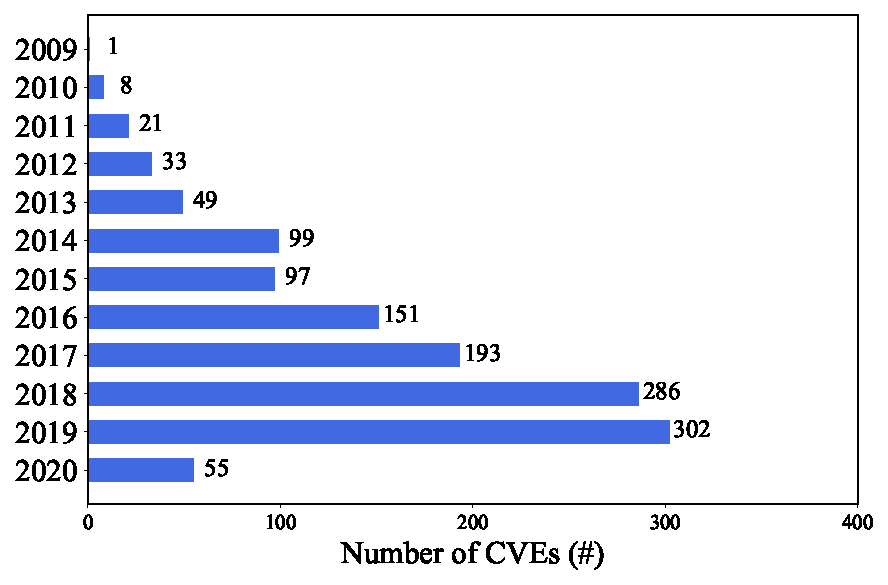
\includegraphics[scale=0.46]{res/rq0-year.pdf}
    %\vspace{-5pt}
    \caption{漏洞年份分布统计}\label{fig:rq0-year}
    \end{subfigure}
    \begin{subfigure}[b]{0.45\textwidth}
    \centering
    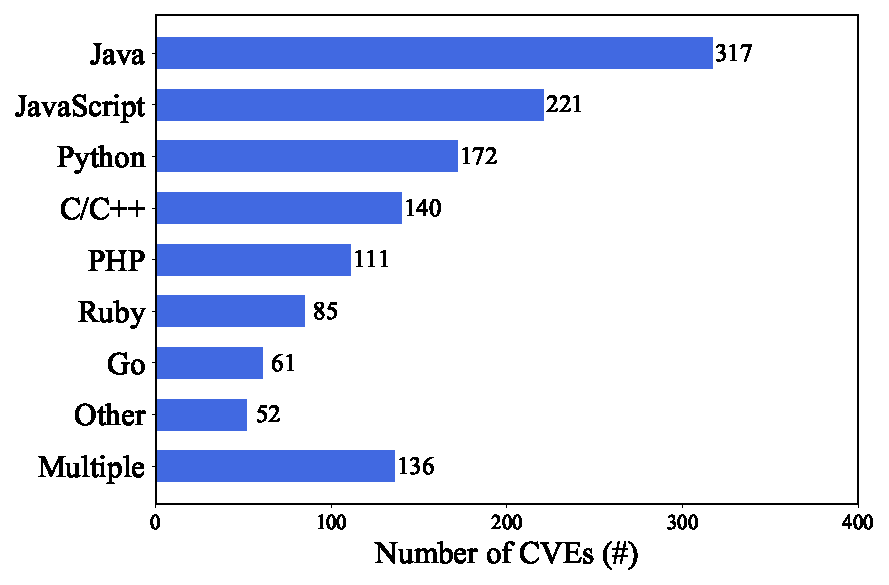
\includegraphics[scale=0.46]{res/rq0-language.pdf}
    %\vspace{-5pt}
    \caption{程序语言分布统计}\label{fig:rq0-language}
    \end{subfigure}
    %\vspace{-20pt}
    \caption{数据集中漏洞年份及程序语言分布统计}\label{fig:dataset}
\end{figure*}

\section{RQ1:覆盖率分析}\label{sec:coverage}

\section{RQ2:一致性分析}\label{sec:consistency}

\section{RQ3:补丁类型分析}\label{sec:type}

\section{RQ4:补丁映射分析}\label{sec:cardinality}

\section{RQ5:补丁准确性分析}\label{sec:accuracy}
